\documentclass[tikz]{standalone}

\usepackage{amsmath}

\usetikzlibrary{arrows.meta,patterns}
%\usetikzlibrary{arrows.meta,backgrounds,fit,positioning}

\begin{document}
	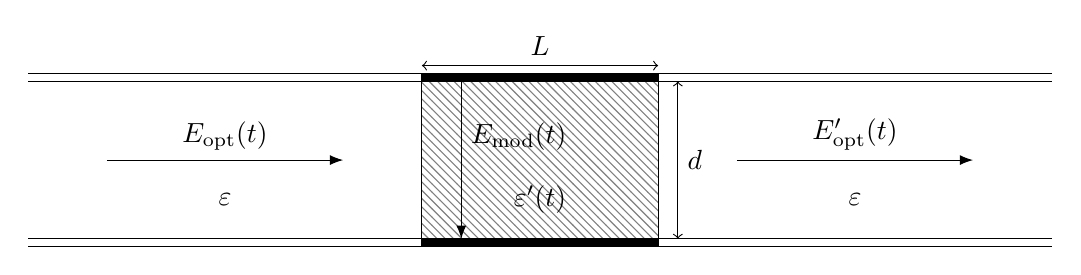
\begin{tikzpicture}
		\coordinate (a) at (0,0);
		\coordinate (c) at (13,2);
		\coordinate (b) at (a-|c);
		\coordinate (d) at (a|-c);
		
		\draw (a) -- (b);
		\draw (c) -- (d);
		\draw (a) ++(0,-0.1) -- ++(13,0);
		\draw (d) ++(0,+0.1) -- ++(13,0);
		
		\draw[pattern=north west lines, pattern color=gray] (5,0) rectangle ++(3,2);		
		
		\node at (2.5,0.5) {$\varepsilon$};
		\node at (10.5,0.5) {$\varepsilon$};
		\node at (6.5,0.5) {$\varepsilon^\prime(t)$};
		
		\draw[fill=black] (5,0) rectangle ++(3,-0.1);
		\draw[fill=black] (5,2) rectangle ++(3,+0.1);
		
		\draw[-Latex] (1,1) -- ++(3,0) node[midway, above]{$E_\text{opt}(t)$};
		\draw[-Latex] (9,1) -- ++(3,0) node[midway, above]{$E^\prime_\text{opt}(t)$};
		\draw[-Latex] (5.5,2) -- ++(0,-2) node[midway, above right]{$E_\text{mod}(t)$};
		\draw[to-to] (8.25,2) -- ++(0,-2) node[midway, right]{$d$};
		\draw[to-to] (5,2.2) -- ++(3,0) node[midway, above]{$L$};
	\end{tikzpicture}
\end{document}
